\documentclass[10pt,twoside]{article}
\usepackage[utf8]{inputenc}
\usepackage{amsmath}
\usepackage{amsfonts}
\usepackage{amssymb}
\usepackage[spanish,es-noshorthands]{babel}
\usepackage[T1]{fontenc}
\usepackage{lmodern}
\usepackage{graphicx,hyperref}
\usepackage{tikz,pgf}
\usepackage{multicol}
\usepackage{subfig}
\usepackage[papersize={6.5in,8.5in},width=5.5in,height=7in]{geometry}
\usepackage{fancyhdr}
\pagestyle{fancy}
\fancyhead[LE]{
\includegraphics[height=12pt]{Images/logo-colegio.png} Matemáticas $6^{\circ}$}
\fancyhead[RE]{}
\fancyhead[RO]{\textit{Germ\'an Avenda\~no Ram\'irez, Lic. U.D., M.Sc. U.N.}}
\fancyhead[LO]{}

\author{Germ\'an Avenda\~no Ram\'irez, Lic. U.D., M.Sc. U.N.}
\title{\begin{minipage}{.2\textwidth}

\includegraphics[height=1.75cm]{Images/logo-colegio.png}\end{minipage}
\begin{minipage}{.55\textwidth}
\begin{center}
Taller Nivelación 2014 \\
Matemáticas $6^{\circ}$
\end{center}
\end{minipage}\hfill
\begin{minipage}{.2\textwidth}

\includegraphics[height=1.75cm]{Images/logo-sed.png} 
\end{minipage}}
\date{}
\begin{document}
\maketitle
Nombre: \hrulefill Curso: \underline{603} Fecha: \underline{\hspace*{2.5cm}}
\section*{N\'{u}meros naturales}
\begin{enumerate}
\item Explique la propiedad distributiva de la multiplicaci\'{o}n con respecto a la suma y resuelva de dos maneras los siguientes productos
\begin{enumerate}
\begin{multicols}{3}
\item $17\cdot 38+17\cdot 12$
\item $96\cdot 59+4\cdot 59$
\item $149\cdot 19+52\cdot 19$
\end{multicols}
\end{enumerate}
\item Saca el factor común en las siguientes expresiones:
\begin{enumerate}
\begin{multicols}{3}
\item $120+130+170$
\item $25+35+50$
\item $48-16+72$
\end{multicols}
\end{enumerate}
\item Resuelva y compruebe:
\begin{enumerate}
\begin{multicols}{3}
\item $(3^{4})^{4}$
\item $(8^{2})^{3}$
\item $(9^{3})^{2}$
\end{multicols}
\end{enumerate}
\item Realice las siguientes operaciones:
\begin{enumerate}
\begin{multicols}{2}
\item $3+6\cdot 5-3\cdot 4-2=$
\item $3+(6+4)\cdot 5-4\cdot 6-3+(2\cdot 8)\div 4=$
\item $7\cdot 3+[6+2\cdot (8\div 4+3\cdot 2)-7\cdot 2]+9\div 3=$
\end{multicols}
\end{enumerate}
\item La suma de dos números es 288 y el cociente entre ellos es 8. ¿Cuáles son los números?
\item Don Tomás quiere repartir unos libros entre sus hijos. Puede hacerlo dándoles 1 al mayor, 2 al segundo, 3 al tercero \ldots Otro modo de repartirlos sería dar 7 a cada uno. ¿Cuántos hijos y cuántos libros tiene don Tomás?
\item El producto de dos números es 64 y su suma 20. ¿Cuáles son eso números?
\item Maité quiere comprar sellos. Tiene menos de 100 pesetas, si los compra todos de 5 pesetas, le sobra una peseta. Si los compra de 8 pesetas le sobran 6 pesetas. Le falta una peseta para comprar un n\'{u}mero exacto de sellos de 29 pesetas. ¿Cu\'{a}nto dinero tiene Mait\'{e}?
\item En una granja se han vendido 1482 huevos. Si dos docenas y media cuestan \$5400. ¿Cuánto valen los huevos?
\item Un camionero carga en su camión 4 televisores y 3 microondas. Si cada televisor pesa como tres microondas y en total ha cargado 75 kilos, ¿cuańto pesa cada aparato?
\section*{Divisibilidad}
\item ¿Cuál es el menor número que tiene por divisores?
\begin{enumerate}
\begin{multicols}{3}
\item 7, 5
\item 2, 6
\item 3, 4, 12
\end{multicols}
\end{enumerate}
\item ¿De cuántas maneras se puede escribir 10 como suma de dos números primos? ¿Y 47? ¿Y 103?
\item El producto de tres números es 360
\begin{enumerate}
\item ¿Cuáles pueden ser estos tres números?
\item ¿Podrías escribir todas las soluciones del problema?
\end{enumerate}
\item Compruebe que para saber si un número menor que 100 es primo, es suficiente con dividir por 2, 3, 5 y 7. ¿Por cuántos números como máximo tendrá que dividir para saber si es primo el número 497?
\item La suma de dos números es igual a 148. Si se divide el mayor por el menor, el cociente es igual a cinco y el resto (residuo) es 10. ¿Cuáles son esos números?
\item ¿Puede haber además del 2 y del 3, otros dos números consecutivos que sean números primos? Justifique su respuesta
\item En una granja se ha recogido un número de huevos entre setecientos y ochocientos. Forman un número exacto de docenas. También se podrían colocar exactamente en cartones de 15 huevos. ¿Cuántos huevos se han recogido en la granja?
\item A un niño le preguntaron que cuánta canicas tenía en un bote, contestó de la siguiente manera: "Ayer las agrupé de 11 en 11 y sobraban 5; hoy las he agrupado de 23 en 23 y sobraban 3. ¿Cuál es el menor número de canicas que puede tener el niño en el bote?
\begin{minipage}{.6\textwidth}
\item Si se eliminan 3 de los doce primeros divisores de 216, se puede conseguir con los otros nueve, sin repetir ninguno el siguiente cuadrado mágico multiplicativo, de manera que el producto de los tres números que ocupan cualquiera de las filas, columnas o diagonales, es siempre 216.
\end{minipage} \hfill
\begin{minipage}{.35\textwidth}
\begin{tikzpicture}
\draw (0,0) grid (3,3);
\node at (1.5,.5){36};
\node at (1.5,1.5){6};
\end{tikzpicture}
\end{minipage}
\section*{Fracciones}
\item En una clase de 24 alumnos, $\frac{5}{8}$ son chicos. ¿Cuántos chicos y chicas hay en clase?
\item El depósito (tanque) de un autom\'{o}vil tiene una capacidad de 63 litros de gasolina, si gasta los $\frac{5}{9}$ en una excursi\'{o}n, ¿cu\'{a}ntos litros le quedan al volver de viaje?
\item Indique cu\'{a}les de las siguientes fracciones dan como resultado un n\'{u}mero natural y cu\'{a}les un n\'{u}mero decimal:
\begin{enumerate}
\begin{multicols}{7}
\item $\dfrac{3}{2}$
\item $\dfrac{12}{3}$
\item $\dfrac{17}{4}$
\item $\dfrac{27}{9}$
\item $\dfrac{14}{6}$
\item $\dfrac{19}{8}$
\item $\dfrac{21}{7}$
\end{multicols}
\end{enumerate}
\item Indique cu\'{a}les de las siguientes fracciones son mayores, menores o iguales a la unidad
\begin{enumerate}
\begin{multicols}{6}
\item $\dfrac{1}{7}$
\item $\dfrac{3}{5}$
\item $\dfrac{9}{9}$
\item $\dfrac{5}{3}$
\item $\dfrac{17}{2}$
\item $\dfrac{2}{9}$
\item $\dfrac{16}{4}$
\item $\dfrac{18}{17}$
\item $\dfrac{5}{5}$
\item $\dfrac{6}{9}$
\item $\dfrac{12}{12}$
\item $\dfrac{10}{9}$
\end{multicols}
\end{enumerate}
\item Ordena de mayor a menor las siguientes fracciones:
\begin{enumerate}
\begin{multicols}{2}
\item $\dfrac{8}{7}$, $\dfrac{9}{8}$, $\dfrac{5}{4}$
\item $\dfrac{4}{5}$, $\dfrac{5}{6}$, $\dfrac{8}{10}$, $\dfrac{3}{4}$
\end{multicols}
\end{enumerate}
\item Escriba dos fracciones equivalentes a cada una de éstas:
\begin{enumerate}
\begin{multicols}{5}
\item $\dfrac{13}{5}$
\item $\dfrac{7}{14}$
\item $\dfrac{5}{2}$
\item $\dfrac{45}{18}$
\item $\dfrac{3}{21}$
\end{multicols}
\end{enumerate}
\item ¿Son equivalentes las parejas de fracciones siguientes?
\begin{enumerate}
\begin{multicols}{3}
\item $\dfrac{15}{4}$ y $\dfrac{75}{35}$
\item $\dfrac{33}{42}$ y $\dfrac{132}{168}$
\item $\dfrac{17}{62}$ y $\dfrac{51}{185}$
\end{multicols}
\end{enumerate}
\item En un campeonato de atletismo uno de los saltadores de altura consigue saltar más de dos metros 13 veces de 52 intentos, su contrincante salta m\'{a}s de 2 metros 11 veces de 44 intentos. ¿Cu\'{a}l de los dos ha ganado?
\item Realice las siguientes operaciones simplificando los resultados cuando se pueda
\begin{enumerate}
\begin{multicols}{3}
\item $\dfrac{3}{4}+\dfrac{5}{6}+\dfrac{6}{8}=$
\item $\dfrac{6}{10}-\dfrac{2}{8}=$
\item $\dfrac{7}{8}+\dfrac{3}{6}-\dfrac{5}{12}=$
\end{multicols}
\end{enumerate}
\item María estudia $\frac{3}{4}$ de hora matemáticas, $\frac{2}{3}$ de hora ciencias naturales, $\frac{4}{6}$ de hora lenguaje y $\frac{3}{8}$ de hora inglés. ¿Cuántas horas estudia María?
\section*{Estad\'{i}stica}
\begin{minipage}{.4\textwidth}
\item El siguiente gr\'{a}fico expresa el n\'{u}mero de refrescos consumidos durante 6 meses en un bar de la capital
\begin{enumerate}
\item ¿Cómo se denomina este tipo de gráfica?
\item ¿En qué mes se consumieron más refrescos?
\item ¿Durante que mes se consumieron menos refrescos?
\item Interprete la gráfica
\end{enumerate}
\end{minipage} \hfill
\begin{minipage}{.55\textwidth}
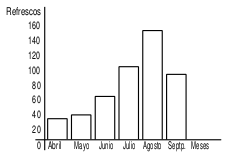
\includegraphics[scale=1]{Images/barras.png} 
\end{minipage}
\item La tabla muestra el número de nacimientos en los siete primeros meses de un año
\begin{center}
\begin{tabular}{|c|c|c|c|c|c|c|c|}
\hline 
mes & enero & febrero & marzo & abril & mayo & junio & julio \\ 
\hline 
No nacimientos & 24 & 31 & 32 & 29 & 32 & 31 & 40 \\ 
\hline 
\end{tabular} 
\end{center}
\begin{enumerate}
\item ¿En qué mes hubo más nacimientos?
\item ¿En qué mes hubos menos nacimientos?
\item ¿Hubo dos meses con el mismo número de nacimientos?
\item ¿Le corresponde a cada mes un único número de nacimientos?
\end{enumerate}
\end{enumerate}
\fbox{\begin{minipage}{.99\textwidth}
\emph{Este trabajo debe ser resuelto en hoja examen y entregado justo antes de la evaluación según horario definido por la institución. Es requisito indispensable para presentar la evaluación, ya que el propósito de éste es preparar los temas esenciales vistos durante el año escolar}
\end{minipage}}
\end{document}
